\section{Results: visible gains and their boundaries}
\subsection{The three primary treatments}
All \ChallengeCalls{} main attempts completed with saved raw responses and no technical failures. There are \ChallengePositives{} positive and \ChallengeNegatives{} zero-optimum cases. Figure~\ref{fig:headline} shows the primary contrast directly. General company context supports 47.9\% of optimal policy value; GTM context supports 88.4\%. GPT returns \GPTCompany\% versus \GPTGTM\%, and Opus returns \OpusCompany\% versus \OpusGTM\%. The paired gains are \GPTGain{} percentage points [\GPTLower, \GPTUpper] and \OpusGain{} [\OpusLower, \OpusUpper]. Both Holm-adjusted random-sign $p$-values are approximately 0.00020, at the Monte Carlo test's resolution. These intervals describe generated company worlds, not a real-company population.

GTM improves the company-mean score in 113 worlds for GPT and 112 for Opus; the remaining worlds tie. It returns a fully supported nonempty plan on 286/288 positive cases for GPT and 284/288 for Opus, versus 202/288 for Company with either reader. All six treatments safely abstain on all 72 zero-optimum cases for each reader. The no-context zero in the primary graph reflects unavailable company evidence, not zero general marketing competence.

\begin{figure}[t]
\centering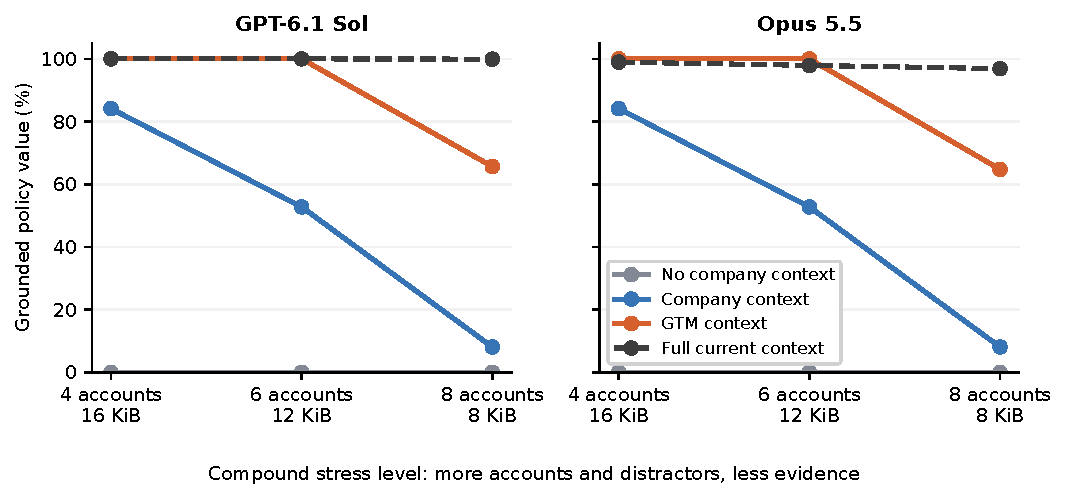
\includegraphics[width=\linewidth]{figures/challenge/difficulty.pdf}
\caption{The gap grows under the compound stress setting: Company falls from 84.1\% to 52.8\% to 8.1\%; GTM reaches 100\%, 100\% and 65.7\% (GPT) or 64.8\% (Opus). Each point contains 96 positive cases. Full current context is an information-rich reference. These settings jointly change accounts, distractions/conflicts and evidence allowance; the curves do not isolate one causal factor.}
\label{fig:difficulty}
\end{figure}

\begin{table}[t]
\centering\footnotesize\begin{tabular}{llrrrr}
\toprule
Reader & Context & Value (\%) & Exact / positive & Unsupported / all & API USD \\
\midrule
GPT-6.1 Sol & None & 0.0 & 0/288 & 0/360 & 1.06 \\
GPT-6.1 Sol & Company & 47.9 & 82/288 & 0/360 & 4.88 \\
GPT-6.1 Sol & GTM & 88.4 & 217/288 & 0/360 & 5.95 \\
GPT-6.1 Sol & Markdown & 45.7 & 73/288 & 0/360 & 4.69 \\
GPT-6.1 Sol & GBrain search & 0.0 & 0/288 & 0/360 & 5.09 \\
GPT-6.1 Sol & Full context & 100.0 & 287/288 & 0/360 & 15.62 \\
\midrule
Opus 5.5 & None & 0.0 & 0/288 & 0/360 & 4.32 \\
Opus 5.5 & Company & 47.9 & 82/288 & 0/360 & 16.06 \\
Opus 5.5 & GTM & 88.2 & 217/288 & 2/360 & 18.50 \\
Opus 5.5 & Markdown & 45.4 & 72/288 & 1/360 & 16.02 \\
Opus 5.5 & GBrain search & 0.0 & 0/288 & 0/360 & 13.40 \\
Opus 5.5 & Full context & 98.1 & 282/288 & 6/360 & 42.08 \\
\bottomrule
\end{tabular}

\caption{Every executed treatment. Value is the equal-company positive score. Exact means the full-information optimum with all required citations. Unsupported counts include any plan-contract violation; all nine observed violations are citation defects on positive cases, not ineligible actions or negative-case recommendations. USD is the observed reader subtotal for 360 calls. The identical-input query-word control adds zero calls.}
\label{tab:results}
\end{table}

\subsection{What stronger generic controls change}
The generic task-word selector produces \emph{the exact ordered evidence and messages} of GTM on 360/360 cases, verified before main generation. It uses shared query words rather than a GTM relation allowlist. Figure~\ref{fig:controls} aliases the corresponding recorded responses and explicitly does not count them as independent observations. Thus the main improvement over unconditioned entity closure does not demonstrate a need for a separate vertical database or proprietary ontology.

Structured Markdown reaches 45.7\% for GPT and 45.4\% for Opus under the main allowances. Full current context reaches \GPTFull\% and \OpusFull\%, respectively. Native GBrain search alone yields no complete eligible chain under these allowances. Its long composite query produced zero lexical matches in all 360 native executions, with real vector retrieval active. This configured search component lacks the full product's adaptive query decomposition, graph ingestion and agent loop. Its score must not be read as a whole-product capability ranking.

\begin{figure}[t]
\centering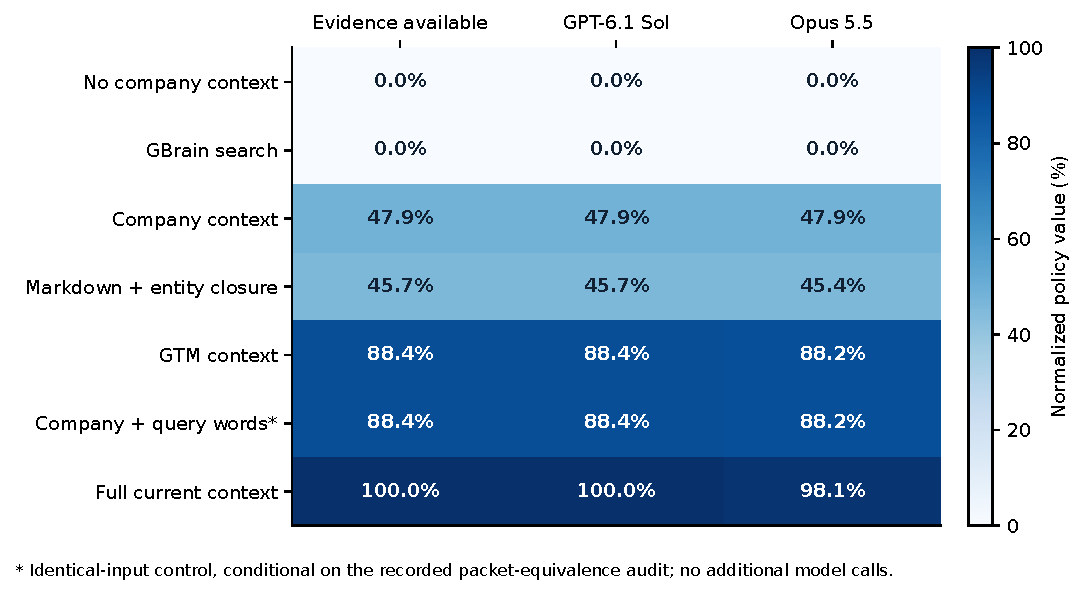
\includegraphics[width=\linewidth]{figures/challenge/controls.pdf}
\caption{All controls, including the generic method that exactly matches the specialized inputs. Evidence and reader value use the same positive denominator. The GBrain search row is a documented component configuration, not a product leaderboard. Full context has a larger input allowance.}
\label{fig:controls}
\end{figure}

The declared retrieval-only sweep further bounds the effect (Figure~\ref{fig:budget}). At 16~KiB, GTM recovers 100\% versus 59.7\% for Company. Company reaches 98.5\% at 64~KiB and 100\% at 128~KiB; every plotted method reaches 100\% at the latter allowance. These are new context computations over the same cases, with \emph{no reader calls} at the alternate budgets. Specialization improves evidence efficiency here; it does not exceed an unlimited generic information reference.

\begin{figure}[t]
\centering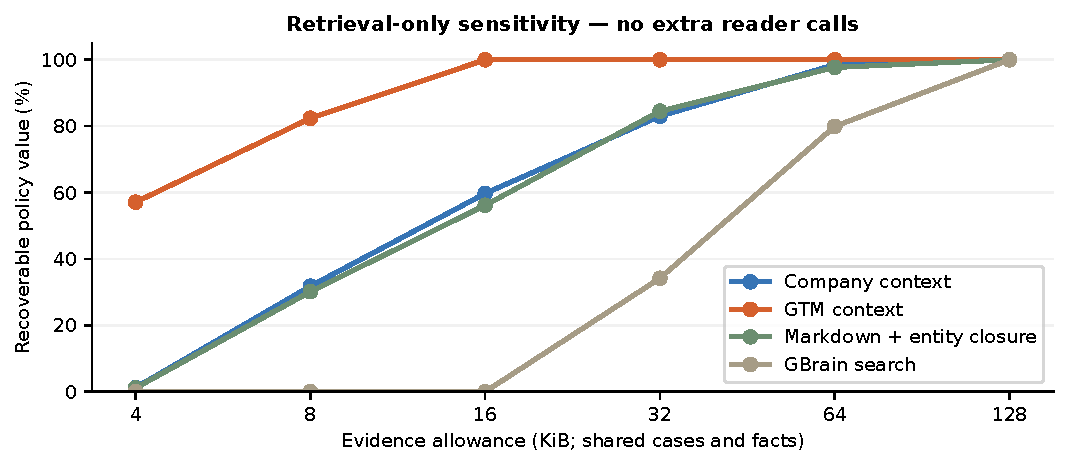
\includegraphics[width=\linewidth]{figures/challenge/budget.pdf}
\caption{Larger generic contexts close the evidence-selection gap. Each point uses all main cases and the equal-company positive aggregation; it is recoverable formal value, not measured recommendation performance at that allowance.}
\label{fig:budget}
\end{figure}

\subsection{Context quality versus reader quality}
Figure~\ref{fig:decomposition} separates missing support from unused support. Both readers attain the context-supported optimum on every Company positive case. GPT falls below its GTM context ceiling once and its full-context ceiling once. Opus has two GTM, one Markdown and six full-context citation failures; all nine plans would otherwise attain their selected context's optimum. Missing bindings concern six priorities, one capacity approval, one proof verification and one initiative-to-need link. No returned plan violates eligibility, the shared resource budget or the distinct-account rule.

A disclosed post-hoc sensitivity removes citation-binding checks while retaining context-supported eligibility and all global constraints. Opus then reaches 88.4\% with GTM and 100\% with full context; GPT scores are unchanged. The primary scores remain unchanged. This diagnosis prevents a citation defect from being misinterpreted as a bad strategic choice, while retaining the strict provenance requirement appropriate to an evidence-backed action interface.

\begin{figure}[t]
\centering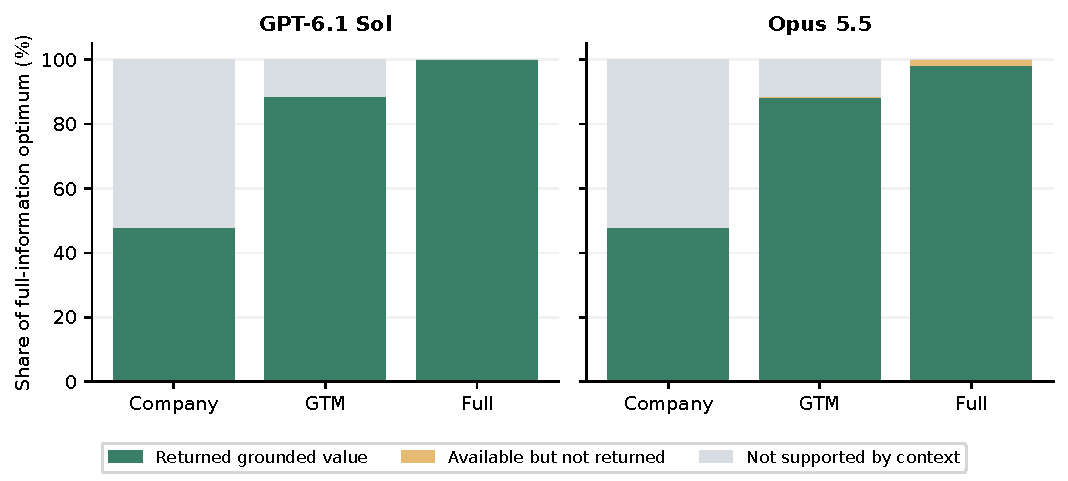
\includegraphics[width=\linewidth]{figures/challenge/decomposition.pdf}
\caption{Where value is lost. Gray is unavailable under the selected evidence; amber is available but not returned with valid citations and constraints; green is realized grounded value. This descriptive decomposition is not causal mediation analysis. Most lost value precedes the reader.}
\label{fig:decomposition}
\end{figure}

\paragraph{Qualitative trace checks.}
We inspect every reader shortfall and retain source IDs, responses and reference plans. In world 001/stress, Company supports no action, GTM only 6/66 possible points, and Markdown 48/66: the aggregate GTM advantage is not a per-case dominance guarantee. In world 000/stress, GTM preserves 30/62 points but still omits useful support. These are the first lexicographic cases of the stated retrieval-failure categories, selected descriptively after the run. In world 097/stress, Opus explicitly notices a wrong priority citation in its prose yet leaves the structured action unchanged; the validator correctly rejects that binding. GPT's world 009/stress full-context plan claims optimality at 95 points while the reference finds 105. These examples are research-assistant analysis, not blinded human judgments.

\subsection{Observed resources}
Main reader usage totals an estimated \$\ChallengeCost{}. Across availability checks, both development stages, the main, the external Opus extension and all new embedding responses, known usage totals \$183.66: 4,958 generation and 539 embedding responses, with no unknown-usage attempts in this new study. The earlier studies have separate accounting and are not included in these totals.

\begin{figure}[t]
\centering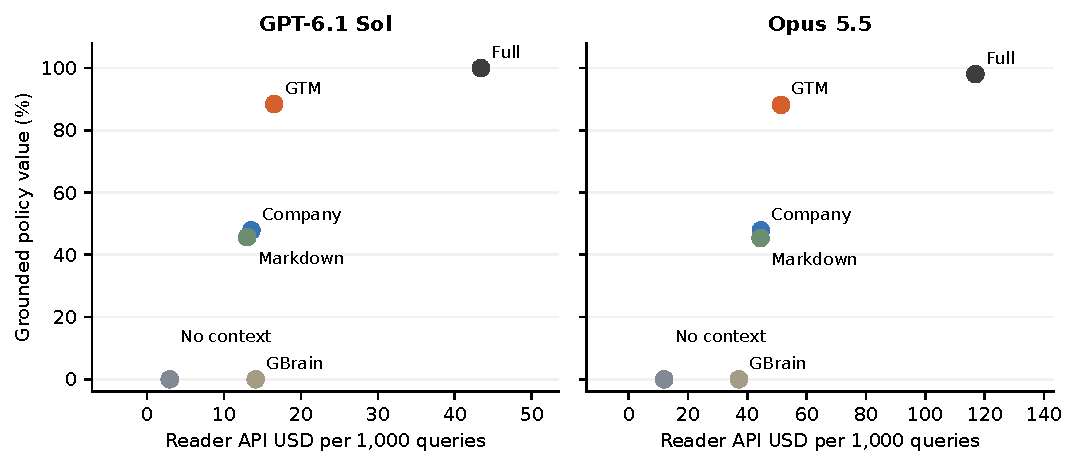
\includegraphics[width=\linewidth]{figures/challenge/cost.pdf}
\caption{Reader value versus realized API usage per 1,000 queries, including the main mix of positive and negative cases. Full context costs more and performs better. Prices, tokenizers, effort and caching differ across providers; within-reader comparisons are the intended interpretation. Ingestion, maintenance, infrastructure and practitioner time are excluded.}
\label{fig:cost}
\end{figure}

GTM slightly increases the reader bill over Company while recovering substantially more formal value. Full context costs 2.63 times GTM for GPT and 2.27 times for Opus. These are observed usage ratios, not general cost guarantees; Table~\ref{tab:resources} supplies token and elapsed-time operating points. The common clean-record boundary and shared embedding cache exclude important production costs. No savings in revenue acquisition or total ownership cost are established.
